% The document class supplies options to control rendering of some standard
% features in the result.  The goal is for uniform style, so some attention 
% to detail is *vital* with all fields.  Each field (i.e., text inside the
% curly braces below, so the MEng text inside {MEng} for instance) should 
% take into account the following:
%
% - author name       should be formatted as "FirstName LastName"
%   (not "Initial LastName" for example),
% - supervisor name   should be formatted as "Title FirstName LastName"
%   (where Title is "Dr." or "Prof." for example),
% - degree programme  should be "BSc", "MEng", "MSci", "MSc" or "PhD",
% - dissertation title should be correctly capitalised (plus you can have
%   an optional sub-title if appropriate, or leave this field blank),
% - dissertation type should be formatted as one of the following:
%   * for the MEng degree programme either "enterprise" or "research" to
%     reflect the stream,
%   * for the MSc  degree programme "$X/Y/Z$" for a project deemed to be
%     X%, Y% and Z% of type I, II and III.
% - year              should be formatted as a 4-digit year of submission
%   (so 2014 rather than the academic year, say 2013/14 say).

\documentclass[ oneside,% the name of the author
                    author={George Herbert},
                % the degree programme: BSc, MEng, MSci or MSc.
                    degree={MSci},
                % the dissertation    title (which cannot be blank)
                     title={Video Diffusion Models for Climate Simulations},
                % the dissertation subtitle (which can    be blank)
                  subtitle={}]{dissertation}

\begin{document}

% =============================================================================

% This macro creates the standard UoB title page by using information drawn
% from the document class (meaning it is vital you select the correct degree 
% title and so on).

\maketitle

% After the title page (which is a special case in that it is not numbered)
% comes the front matter or preliminaries; this macro signals the start of
% such content, meaning the pages are numbered with Roman numerals.

\frontmatter


%\lstlistoflistings

% The following sections are part of the front matter, but are not generated
% automatically by LaTeX; the use of \chapter* means they are not numbered.

% -----------------------------------------------------------------------------

\chapter*{Abstract}

% {\bf A compulsory section, of at most 300 words} 
% \vspace{1cm} 

% \noindent
% This section should pr\'{e}cis the project context, aims and objectives,
% and main contributions (e.g., deliverables) and achievements; the same 
% section may be called an abstract elsewhere.  The goal is to ensure the 
% reader is clear about what the topic is, what you have done within this 
% topic, {\em and} what your view of the outcome is.

% The former aspects should be guided by your specification: essentially 
% this section is a (very) short version of what is typically the first 
% chapter. If your project is experimental in nature, this should include 
% a clear research hypothesis.  This will obviously differ significantly
% for each project, but an example might be as follows:

% \begin{quote}
% My research hypothesis is that a suitable genetic algorithm will yield
% more accurate results (when applied to the standard ACME data set) than 
% the algorithm proposed by Jones and Smith, while also executing in less
% time.
% \end{quote}

% \noindent
% The latter aspects should (ideally) be presented as a concise, factual 
% bullet point list.  Again the points will differ for each project, but 
% an might be as follows:

% \begin{quote}
% \noindent
% \begin{itemize}
% \item I spent $120$ hours collecting material on and learning about the 
%       Java garbage-collection sub-system. 
% \item I wrote a total of $5000$ lines of source code, comprising a Linux 
%       device driver for a robot (in C) and a GUI (in Java) that is 
%       used to control it.
% \item I designed a new algorithm for computing the non-linear mapping 
%       from A-space to B-space using a genetic algorithm, see page $17$.
% \item I implemented a version of the algorithm proposed by Jones and 
%       Smith in [6], see page $12$, corrected a mistake in it, and 
%       compared the results with several alternatives.
% \end{itemize}
% \end{quote}

% -----------------------------------------------------------------------------


\chapter*{Dedication and Acknowledgements}

% {\bf A compulsory section}
% \vspace{1cm} 

% \noindent
% It is common practice (although totally optional) to acknowledge any
% third-party advice, contribution or influence you have found useful
% during your work.  Examples include support from friends or family, 
% the input of your Supervisor and/or Advisor, external organisations 
% or persons who  have supplied resources of some kind (e.g., funding, 
% advice or time), and so on.


% -----------------------------------------------------------------------------

% This macro creates the standard UoB declaration; on the printed hard-copy,
% this must be physically signed by the author in the space indicated.

\makedecl



% -----------------------------------------------------------------------------

% LaTeX automatically generates a table of contents, plus associated lists 
% of figures and tables.  These are all compulsory parts of the dissertation.

\tableofcontents
\listoffigures
\listoftables

% -----------------------------------------------------------------------------



\chapter*{Ethics Statement}

% {\bf A compulsory section} 
% \vspace{1cm} 

% In almost every project, this will be one of the following statements:
%     \begin{itemize}
%         \item ``This project did not require ethical review, as determined by my supervisor, [fill in name]''; or
%         \item ``This project fits within the scope of ethics application 0026, as reviewed by my supervisor, [fill in name]''; or
%         \item ``An ethics application for this project was reviewed and approved by the faculty research ethics committee as application [fill in number]''.
%     \end{itemize}
    
% See Section 3.2 of the unit Handbook for more information. If something went wrong and none of those three statements apply, then you should instead explain what happened.


% -----------------------------------------------------------------------------

% \chapter*{Supporting Technologies}

% {\bf An optional section}
% \vspace{1cm} 

% \noindent
% This section should present a detailed summary, in bullet point form, 
% of any third-party resources (e.g., hardware and software components) 
% used during the project.  Use of such resources is always perfectly 
% acceptable: the goal of this section is simply to be clear about how
% and where they are used, so that a clear assessment of your work can
% result.  The content can focus on the project topic itself (rather,
% for example, than including ``I used \mbox{\LaTeX} to prepare my 
% dissertation''); an example is as follows:

% \begin{quote}
% \noindent
% \begin{itemize}
% \item I used the Java {\tt BigInteger} class to support my implementation 
%       of RSA.
% \item I used a parts of the OpenCV computer vision library to capture 
%       images from a camera, and for various standard operations (e.g., 
%       threshold, edge detection).
% \item I used an FPGA device supplied by the Department, and altered it 
%       to support an open-source UART core obtained from 
%       \url{http://opencores.org/}.
% \item The web-interface component of my system was implemented by 
%       extending the open-source WordPress software available from
%       \url{http://wordpress.org/}.
% \end{itemize}
% \end{quote}

% -----------------------------------------------------------------------------

\chapter*{Notation and Acronyms}

% {\bf An optional section}
% \vspace{1cm} 

% \noindent
% Any well written document will introduce notation and acronyms before
% their use, {\em even if} they are standard in some way: this ensures 
% any reader can understand the resulting self-contained content.  

% Said introduction can exist within the dissertation itself, wherever 
% that is appropriate.  For an acronym, this is typically achieved at 
% the first point of use via ``Advanced Encryption Standard (AES)'' or 
% similar, noting the capitalisation of relevant letters.  However, it 
% can be useful to include an additional, dedicated list at the start 
% of the dissertation; the advantage of doing so is that you cannot 
% mistakenly use an acronym before defining it.  A limited example is 
% as follows:

\begin{quote}
\noindent
\begin{tabular}{lcl}
%      $\mathbf{X}\circ\mathbf{Y}$ &: & Hadamard product (i.e. element-wise product) of matrices $\mathbf{X}$ and $\mathbf{Y}$\\
      i.i.d. &: & Independent and identically distributed\\
      KL &: & Kullback--Leibler\\
      VAE &: & Variational Autoencoder\\
      &\vdots&\\
      $\mathbf{X}^{\circ n}$ &: & Element-wise exponentiation of matrix $\mathbf{X}$ with power $n$\\
      $\mathrm{diag}(\mathbf{x})$ &: & Diagonal matrix with the values of vector $\mathbf{x}$ on the diagonal\\
      $\log(x)$ &: & Natural logarithm function (i.e. logarithm with base $e$) applied to $x$\\
      $f\simeq g$ &: & $g$ is an unbiased estimator of $f$\\
     
% AES                 &:     & Advanced Encryption Standard                                         \\
% DES                 &:     & Data Encryption Standard                                             \\
%                     &\vdots&                                                                      \\
% ${\mathcal H}( x )$ &:     & the Hamming weight of $x$                                            \\
% ${\mathbb  F}_q$    &:     & a finite field with $q$ elements                                     \\
% $x_i$               &:     & the $i$-th bit of some binary sequence $x$, st. $x_i \in \{ 0, 1 \}$ \\
\end{tabular}
\end{quote}


% =============================================================================

% After the front matter comes a number of chapters; under each chapter,
% sections, subsections and even subsubsections are permissible.  The
% pages in this part are numbered with Arabic numerals.  Note that:
%
% - A reference point can be marked using \label{XXX}, and then later
%   referred to via \ref{XXX}; for example Chapter\ref{chap:context}.
% - The chapters are presented here in one file; this can become hard
%   to manage.  An alternative is to save the content in seprate files
%   the use \input{XXX} to import it, which acts like the #include
%   directive in C.

\mainmatter


\chapter{Introduction}
\label{chap:introduction}

\chapter{Background}
\label{chap:background}

\section{Generative Models}
\label{sec:background_generative}

Let us consider some dataset $\mathcal{D}$ consisting of $N_{\mathcal{D}}\ge1$ datapoints which we assume are independent and identically distributed (i.i.d.):
\begin{align}
      \mathcal{D}=\{\mathbf{x}^{(i)}\mid 1 \le i \le N_{\mathcal{D}}, i \in \mathbb{N} \}
\end{align}
We assume each observed datapoint $\mathbf{x}\in\mathcal{D}$ is a random sample from an underlying process, whose true distribution $p^*(\mathbf{x})$ is unknown. The goal of \textit{generative modelling} is to approximate this true distribution with a chosen model $p_\theta(\mathbf{x})$ with parameters $\theta$. We learn parameters $\mathbf{\theta}$ such that the probability distribution function given by the model $p_\theta(\mathbf{x})$ approximates the true distribution of the data, such that for any observed $\mathbf{x}\in\mathcal{D}$, we have:
\begin{align}
      p_\theta(\mathbf{x}) \approx p^*(\mathbf{x})
\end{align}
Once learned, we can \textit{generate} new samples unconditionally from our approximate model at will.

\section{Latent Variables}
\label{sec:background_latent}

We can think of each observed datapoint $\mathbf{x}\in\mathcal{D}$ as being represented or generated via one or more associated \textit{latent variables} $\mathbf{z}$. The latent variables are part of the model, but we do not observe them directly, and they are not within the dataset. We model the joint distribution of the observed data $\mathbf{x}$ and the latent variables $\mathbf{z}$ by $p_\theta(\mathbf{x},\mathbf{z})$; the marginal distribution over the observed variable $p_\theta(\mathbf{x})$ is given by:
\begin{align}
      p_\theta(\mathbf{x})=\int p_\theta(\mathbf{x},\mathbf{z}) d\mathbf{z}
\end{align}
In this work, the conditional dependencies between the observed variable $\mathbf{x}$ and the latent variables $\mathbf{z}$ are either parameterised using a neural network or explicitly defined. 

\section{Variational Autoencoders}
\label{sec:background_vae}

% The broader literature contains several well-known approaches to learning a model $p_\theta(\mathbf{x})$. Likelihood-based generative modelling, for example, seeks to learn a model that assigns a high likelihood to the observed datapoints $\mathcal{D}$. Variational autoencoders (VAEs) \cite{Autoencoding_Variational_Bayes_Kingma,Stochastic_Backpropagation_Rezende} are one such type of likelihood-based generative model.

\subsection{Overview}
\label{sec:background_vae_latent}

The variational autoencoder (VAE) \cite{Autoencoding_Variational_Bayes_Kingma,Stochastic_Backpropagation_Rezende} is one example of a model that utilises latent variables. In its simplest form, the VAE is a latent-variable model $p_\theta(\mathbf{x},\mathbf{z})$ with a single latent $\mathbf{z}$. We assume that each observed variable $\mathbf{x}\in\mathcal{D}$ is generated via a two-step process. First, a latent $\mathbf{z}$ is generated from some true prior distribution $p^*(\mathbf{z})$, followed by an observed value $\mathbf{x}$ generated from some true conditional distribution $p^*(\mathbf{x}|\mathbf{z})$. 

ur model takes the form:
\begin{align}
      p_\theta(\mathbf{x},\mathbf{z})=p_\theta(\mathbf{z})p_\theta(\mathbf{x}|\mathbf{z})
\end{align}
The prior $p_\theta(\mathbf{z})$ over the latent variable is often chosen to be the multivariate standard Gaussian:
\begin{align}
      p_\theta(\mathbf{z})=\mathcal{N}(\mathbf{z};\mathbf{0}, \mathbf{I})
\end{align}
The true posterior $p_\theta(\mathbf{z}|\mathbf{x})$ is intractable, but we commonly assume it takes on the form of a multivariate Gaussian with diagonal covariance. As such, we introduce an a variational approximate posterior, defined as:
\begin{align}
      q_\phi(\mathbf{z}|\mathbf{x})=\mathcal{N}(\mathbf{z}, \boldsymbol{\mu}_\phi(\mathbf{z}), \mathrm{diag}(\boldsymbol\sigma_\phi(\mathbf{z}))^{\circ 2})
\end{align}
with variational parameters $\phi$.

$p_\theta(\mathbf{x}|\mathbf{z})$ and $q_\phi(\mathbf{z}|\mathbf{x})$ are often referred to as the \textit{decoder} and \textit{encoder}, respectively.

\begin{figure}[htbp]
      \centering
      \begin{tikzpicture}[->, >=stealth', auto, node distance=3cm, main node/.style={circle, draw, minimum size=1.25cm}]

            % Nodes
            \node[main node] (x) {$\mathbf{x}$};
            \node[main node, right of=x] (z) {$\mathbf{z}$};
      
            % Edges
            \path[]
            (x) edge [bend left, dashed] node[above] {$q_\phi(\mathbf{z}|\mathbf{x})$} (z)
            (z) edge [bend left] node[below] {$p_\theta(\mathbf{x}|\mathbf{z})$} (x);
      \end{tikzpicture}
      \caption{Graphical depiction of a VAE}
      \label{fig:vae}
\end{figure}


\subsection{Evidence Lower Bound Objective}
\label{sec:background_vae_elbo}

As mentioned in Section \ref{sec:background_generative}, the goal of a generative model, such as a VAE, is to learn parameters $\theta$ such that $p_\theta(\mathbf{x})\approx p^*(\mathbf{x})$. One way to represent this is as a minimisation problem. Mathematically, we wish to learn parameters $\theta$ that minimise the Kullback--Leibler (KL) divergence of the true distribution $p^*(\mathbf{x})$ from our model distribution $p_\theta(\mathbf{x})$, which gives us:
\begin{align}
      \operatorname{argmin}_{\theta} D_{KL}(p^*(\mathbf{x})\Vert p_\theta(\mathbf{x}))&=\operatorname{argmin}_{\theta}\mathbb{E}_{\mathbf{x}\sim p^*(\mathbf{x})}\left[\log\left(\frac{p^*(\mathbf{x})}{p_\theta(\mathbf{x})}\right)\right]\\
      &=\operatorname{argmin}_{\theta}\left(\mathbb{E}_{\mathbf{x}\sim p^*(\mathbf{x})}\left[\log p^*(\mathbf{x})\right]+\mathbb{E}_{\mathbf{x}\sim p^*(\mathbf{x})}\left[-\log p_\theta(\mathbf{x})\right]\right)\\
      &=\operatorname{argmin}_{\theta}\mathbb{E}_{\mathbf{x}\sim p^*(\mathbf{x})}\left[-\log p_\theta(\mathbf{x})\right]
\end{align}
As such, minimisation of the KL divergence equates to minimisation of the negative log-likelihood of our model distribution $p_\theta(\mathbf{x})$ over $\mathbf{x}\sim p^*(\mathbf{x})$. We can analogously express this as maximisation of the log-likelihood:
\begin{align}
      \operatorname{argmax}_{\theta}\mathbb{E}_{\mathbf{x}\sim p^*(\mathbf{x})}\left[\log p_\theta(\mathbf{x})\right]
\end{align}
Moreover, under the assumption that each of the $N_\mathcal{D}$ samples in our dataset $\mathcal{D}$ are i.i.d. according to $p^*(\mathbf{x})$, we have:
\begin{align}
      \mathbb{E}_{\mathbf{x}\sim p^*(\mathbf{x})}\left[\log p_\theta(\mathbf{x})\right]\simeq \frac{1}{N_{\mathcal{D}}}\log p_\theta(\mathcal{D}) = \frac{1}{N_{\mathcal{D}}} \sum_{\mathbf{x}\in\mathcal{D}} \log p_\theta(\mathbf{x})
\end{align}
In other words, under the i.i.d assumption of $\mathcal{D}$, the mean log-likelihood of our model over $\mathcal{D}$ is an unbiased estimator of the expected log-likelihood of our model over $\mathbf{x}\sim p^*(\mathbf{x})$. In practice, for computational efficiency reasons---as well as GPU memory limitations---we learn via mini-batches $\mathcal{M}\subset \mathcal{D}$ of size $N_\mathcal{M} < N_\mathcal{D}$:
\begin{align}
      \frac{1}{N_\mathcal{D}}\log p_\theta(\mathcal{D})\simeq \frac{1}{N_\mathcal{M}}\log p_\theta(\mathcal{M})=\frac{1}{N_\mathcal{M}}\sum_{\mathbf{x}\in\mathcal{M}}\log p_\theta(\mathbf{x})
\end{align}
As such, by transitivity the mean log-likelihood of our model over each mini-batch $\mathcal{M}$ is itself an unbiased estimator of the expected log-likelihood of our model over $\mathbf{x}\sim p^*(\mathbf{x})$.


Firstly, we cannot simply marginalise out the latent variable $\mathbf{z}$ via:
\begin{align}
      p_\theta(\mathbf{x})=\int p_\theta(\mathbf{x},\mathbf{z})d\mathbf{z}
\end{align}
since the integral does not have an analytic solution or efficient estimator. Secondly, we cannot appeal to the chain rule of probability:
\begin{align}
      p_\theta(\mathbf{x})=\frac{p_\theta(\mathbf{x},\mathbf{z})}{p_\theta(\mathbf{z}|\mathbf{x})}
\end{align}
since it requires access to a ground truth latent encoder $p_\theta(\mathbf{z}|\mathbf{x})$.



\begin{align}
      \log p_\theta(\mathbf{x})&=\mathbb{E}_{\mathbf{z}\sim q(\mathbf{z}|\mathbf{x})}\left[\log p_\theta(\mathbf{x})\right]\\
      &=\mathbb{E}_{\mathbf{z}\sim q(\mathbf{z}|\mathbf{x})}\left[\log\left(\frac{p_\theta(\mathbf{x},\mathbf{z})}{p_\theta(\mathbf{z}|\mathbf{x})}\right)\right]\\
      &=\mathbb{E}_{\mathbf{z}\sim q(\mathbf{z}|\mathbf{x})}\left[\log\left(\frac{p_\theta(\mathbf{x},\mathbf{z})q(\mathbf{z}|\mathbf{x})}{p_\theta(\mathbf{z}|\mathbf{x})q(\mathbf{z}|\mathbf{x})}\right)\right]\\
      &=\mathbb{E}_{\mathbf{z}\sim q(\mathbf{z}|\mathbf{x})}\left[\log\left(\frac{p_\theta(\mathbf{x},\mathbf{z})}{q(\mathbf{z}|\mathbf{x})}\right)\right]+\mathbb{E}_{\mathbf{z}\sim q(\mathbf{z}|\mathbf{x})}\left[\log\left(\frac{q(\mathbf{z}|\mathbf{x})}{p_\theta(\mathbf{z}|\mathbf{x})}\right)\right]\\
      &=\mathbb{E}_{\mathbf{z}\sim q(\mathbf{z}|\mathbf{x})}\left[\log\left(\frac{p_\theta(\mathbf{x},\mathbf{z})}{q(\mathbf{z}|\mathbf{x})}\right)\right]+D_{KL}(q(\mathbf{z}|\mathbf{x})\Vert p_\theta(\mathbf{z}|\mathbf{x}))\\
      &\ge \mathbb{E}_{\mathbf{z}\sim q(\mathbf{z}|\mathbf{x})}\left[\log\left(\frac{p_\theta(\mathbf{x},\mathbf{z})}{q(\mathbf{z}|\mathbf{x})}\right)\right]
\end{align}


\subsection{Markovian Hierarchical Variational Autoencoders}
\label{sec:background_vae_hierarchical}

\begin{figure}[htbp]
      \centering
      \begin{tikzpicture}[->, >=stealth', auto, node distance=3cm, main node/.style={circle, draw, minimum size=1.25cm}]

            % Nodes
            \node[main node] (x) {$\mathbf{x}$};
            \node[main node, right of=x] (z1) {$\mathbf{z_1}$};
            \node[main node, right of=z1] (z2) {$\mathbf{z_2}$};
            \node[main node, right of=z2] (z3) {$\mathbf{z_3}$};

            % Edges
            \path[]
            (x) edge [bend left, dashed] node[above] {$q_\phi(\mathbf{z_1}|\mathbf{x})$} (z1)
            (z1) edge [bend left] node[below] {$p_\theta(\mathbf{x}|\mathbf{z_1})$} (x)
            (z1) edge [bend left, dashed] node[above] {$q_\phi(\mathbf{z_2}|\mathbf{z_1})$} (z2)
            (z2) edge [bend left] node[below] {$p_\theta(\mathbf{z_1}|\mathbf{z_2})$} (z1)
            (z2) edge [bend left, dashed] node[above] {$q_\phi(\mathbf{z_3}|\mathbf{z_2})$} (z3)
            (z3) edge [bend left] node[below] {$p_\theta(\mathbf{z_2}|\mathbf{z_3})$} (z2);
      \end{tikzpicture}
      \caption{Graphical depiction of a hierarchical VAE}
      \label{fig:hvae}
\end{figure}


\section{Diffusion Models}
\label{sec:background_diffusion}

Diffusion models are 

Given observed datapoints $\mathbf{x}$, the goal of a generative model is to learn to model its true data distribution $q(\mathbf{x})$.

\subsection{Forward Diffusion Process}
\label{sec:background_diffusion_forward}

The \textit{forward diffusion process} is a Gaussian diffusion process that defines a sequence of increasingly noisy versions of $\mathbf{x}$, which we call the \textit{latent variables}:
\begin{align}
      \mathbf{z}=\{\mathbf{z}_t\mid t\in[0,1]\}
\end{align}
The forward process forms a conditional joint distribution $q(\mathbf{z}|\mathbf{x})$, whose marginal distributions of latent variables $\mathbf{z}_t$ given $\mathbf{x}\sim q(\mathbf{x})$ are given by:
\begin{align}
      q(\mathbf{z}_t|\mathbf{x})=\mathcal{N}\left(\mathbf{z}_t;\alpha_t\mathbf{x},\sigma_t^2\mathbf{I}\right)
      \label{eq:q_z_t_given_x}
\end{align}
where $\alpha_t$ and $\sigma_t$ are strictly positive scalar-valued functions of $t$. The joint distribution of latent variables $\mathbf{z}_r,\mathbf{z}_s,\mathbf{z}_t$ at subsequent timesteps $0\le r < s < t \le 1$ is Markovian:
\begin{align}
      q(\mathbf{z}_t|\mathbf{z}_s,\mathbf{z}_r)&=q(\mathbf{z}_t|\mathbf{z}_s)=\mathcal{N}\left(\mathbf{z}_t; \alpha_{t|s}\mathbf{z}_s, \sigma_{t|s}^2\mathbf{I}\right)
\end{align}
where $\alpha_{t|s}=\alpha_t\alpha_s^{-1}$ and $\sigma_{t|s}^2=\sigma_t^2-\alpha_{t|s}^2\sigma_s^2$. A full derivation of $q(\mathbf{z}_t|\mathbf{z}_s)$ is given in Appendix \ref{appx:diffusion_q_z_t_given_z_s}.

\subsection{Noise Schedule}
\label{sec:background_diffusion_noise_schedule}

We formalise the notion that $\mathbf{z}_t$ is increasingly noisy by defining the log signal-to-noise ratio
\begin{align}
      \lambda_t = \log\left( \frac{\alpha_t^2}{\sigma_t^2}\right)\in[\lambda_{\min}, \lambda_{\max}]
\end{align}
as a strictly monotonically decreasing function $f_{\lambda}$ of time $t\in[0, 1]$, known as the \textit{noise schedule}.

In this work, we use a truncated continuous-time version of the $\alpha$-cosine schedule \cite{IDDPM_Nichol}, introduced in its original discrete-time form by Nichol and Dhariwal \cite{IDDPM_Nichol}. The $\alpha$-cosine schedule was motivated by the fact that the `linear' schedule introduced in prior work by Ho et al. \cite{DDPM_Ho} causes $\alpha_t$ to fall to zero more quickly than is optimal. Nichol and Dhariwal empirically found that this induces too much noise in the latter stages of the forward diffusion process; as such, the latent variables $\mathbf{z}_t$ in these stages contribute little to sample quality. In response, they proposed the original discrete-time $\alpha$-cosine schedule. In this work, we use a continuous-time diffusion model and therefore use an adapted model described in \cite{Simple_Diffusion_Hoogeboom}. More formally, we define:
\begin{align}
      f_{\lambda}(t)=-2\log\left(\tan\left(\frac{\pi}{2}(t_0+t(t_1-t_0))\right)\right)
      \label{eq:f_lambda_alpha_cosine}
\end{align} 
where $t_0$ and $t_1$ truncate $f_{\lambda}(t)$ to the desired range $[\lambda_{\min}, \lambda_{\max}]$ for $t\in[0,1]$, and are themselves defined as:
\begin{align}
      t_0&=\frac{2}{\pi}\arctan\left(\exp\left(-\frac{1}{2}\lambda_{\max}\right)\right)\\
      t_1&=\frac{2}{\pi}\arctan\left(\exp\left(-\frac{1}{2}\lambda_{\min}\right)\right)
\end{align}
Figure \ref{fig:cosine_lambda_t} visualises how the log signal-to-noise ratio $\lambda_t\in[\lambda_{\min},\lambda_{\max}]$ varies with time $t\in[0,1]$ using the $\alpha$-cosine schedule detailed above.

\begin{figure}[htbp]
      \centering
      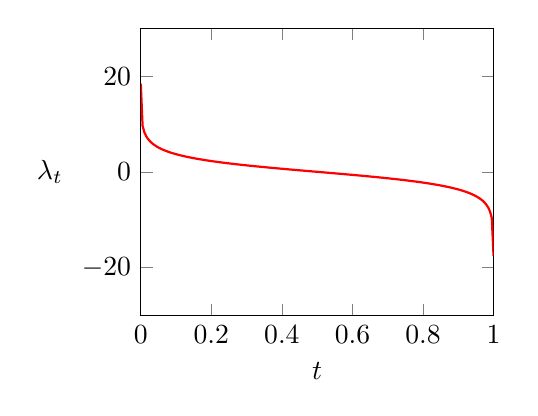
\begin{tikzpicture}
      \begin{axis}[
            xlabel=$t$,
            ylabel=$\lambda_t$,
            ylabel near ticks,
            xlabel near ticks,
            ylabel style={rotate=-90},
            xmin=0,
            xmax=1,
            ymin=-30,
            ymax=30,
            width=.5\linewidth]
      \addplot[color=red,thick,domain=-0.005:1.005,samples=200]{-2 * ln(tan(deg(pi / 2 * ((2 / pi * rad(atan(exp(-0.5 * 30)))) + x * ((2 / pi * rad(atan(exp(-0.5 * -30)))) - (2 / pi * rad(atan(exp(-0.5 * 30)))))))))};
      \end{axis}
      \end{tikzpicture}
      \caption{Relationship between time $t$ and the log signal-to-noise ratio $\lambda_t$ for the truncated continuous-time $\alpha$-cosine noise schedule $f_\lambda(t)$ as defined in Equation \ref{eq:f_lambda_alpha_cosine} with $\lambda_{\min}=-30$ and $\lambda_{\max}=30$. The horizontal axis is time $t\in[0,1]$; the vertical axis is $\lambda_t=f_\lambda(t)\in[\lambda_{\min},\lambda_{\max}]=[-30, 30]$.}
      \label{fig:cosine_lambda_t}
\end{figure}

We can compute $\alpha_t$ and $\sigma_t$ from either $\lambda_t$ or $t$ via the following equations:
\begin{alignat}{2}
      \alpha_t&=\sqrt{S(\lambda_t)}&&=\cos\left(\frac{\pi}{2}(t_0+t(t_1-t_0)\right)\label{eq:alpha_t_alpha_cosine}\\
      \sigma_t&=\sqrt{S(-\lambda_t)}&&=\sin\left(\frac{\pi}{2}(t_0+t(t_1-t_0)\right)\label{eq:sigma_t_alpha_cosine}
\end{alignat}
where $S$ is the sigmoid function. Figure \ref{fig:cosine_alpha_sigma} visualises how the values of $\alpha_t$ and $\sigma_t$ vary with time $t\in[0,1]$ using the $\alpha$-cosine schedule detailed above. Appendix \ref{appx:diffusion_cosine_noise_schedule} provides further details on the form of $f_\lambda$ and how we can derive the forms for $\alpha_t$ and $\sigma_t$.

\begin{figure}[htbp]
      \begin{subfigure}{0.5\textwidth}
            \begin{tikzpicture}
            \begin{axis}[
                  xlabel=$t$,
                  ylabel=$\alpha_t$,
                  ylabel near ticks,
                  xlabel near ticks,
                  ylabel style={rotate=-90},
                  xmin=0,
                  xmax=1,
                  ymin=0,
                  ymax=1,
                  width=\linewidth]
            \addplot[color=red,thick,domain=0:1,samples=100]{cos(deg(pi / 2 * ((2 / pi * rad(atan(exp(-0.5 * 30)))) + x * ((2 / pi * rad(atan(exp(-0.5 * -30)))) - (2 / pi * rad(atan(exp(-0.5 * 30))))))))};
            \end{axis}
            \end{tikzpicture}
      \end{subfigure}
      \begin{subfigure}{0.5\textwidth}
            \begin{tikzpicture}
            \begin{axis}[
                  xlabel=$t$,
                  ylabel=$\sigma_t$,
                  ylabel near ticks,
                  xlabel near ticks,
                  ylabel style={rotate=-90},
                  xmin=0,
                  xmax=1,
                  ymin=0,
                  ymax=1,
                  width=\linewidth]
            \addplot[color=red,thick,domain=0:1,samples=100]{sin(deg(pi / 2 * ((2 / pi * rad(atan(exp(-0.5 * 30)))) + x * ((2 / pi * rad(atan(exp(-0.5 * -30)))) - (2 / pi * rad(atan(exp(-0.5 * 30))))))))};
            \end{axis}
            \end{tikzpicture}
      \end{subfigure}
      \caption{Relationship between time $t$ and $\alpha_t$ (left) and $\sigma_t$ (right) for the same truncated continuous-time $\alpha$-cosine noise schedule as that in Figure \ref{fig:cosine_lambda_t}. The horizontal axis is time $t\in[0,1]$; the vertical axis is the value of $\alpha_t$ (left) and $\sigma_t$ (right).}
      \label{fig:cosine_alpha_sigma}
\end{figure}

\subsection{Generative Model}
\label{sec:background_diffusion_reverse}

The \textit{generative model} is a learned hierarchical model that matches the forward process running in reverse-time: in $T$ uniformly-spaced discrete timesteps, we sequentially generate latent variables, starting from $t=1$ and working backwards to $t=0$. More formally, our hierarchical generative model defines a joint distribution over latent variables:
\begin{align}
      p_\theta(\mathbf{z})=p_\theta(\mathbf{z}_1)\prod_{i=1}^T p_\theta(\mathbf{z}_{s(i)}|\mathbf{z}_{t(i)})
\end{align}
where $s(i)=(i - 1)\cdot T^{-1}$ and $t(i)=i\cdot T^{-1}$. For large enough $\lambda_{\max}$, $\mathbf{z}_0$ is almost noiseless, so learning a model $p_\theta(\mathbf{z}_0)$ is practically equivalent to learning a model $p_\theta(\mathbf{x})$. 

For sufficiently small $\lambda_{\min}$, $\mathbf{z}_1$ contains almost no information about $\mathbf{x}$. As such, there exists a distribution $p_\theta(\mathbf{z}_1)$ such that:
\begin{align}
      D_{KL}(q(\mathbf{z}_1|\mathbf{x})\Vert p_\theta(\mathbf{z_1}))\approx 0
\end{align}
where $D_{KL}$ is the Kullback--Leibler divergence. In this work, we use a variance-preserving diffusion model (i.e. $\alpha_t^2=1-\sigma_t^2$), and as such, we model $p_\theta(\mathbf{z}_1)$ as the multivariate standard Gaussian:
\begin{align}
      p_\theta(\mathbf{z}_1)=\mathcal{N}(\mathbf{z}_1;\mathbf{0}, \mathbf{I})
\end{align}

Once we have sampled $\mathbf{z}_1\sim p_\theta(\mathbf{z}_1)$, we use the discrete-time ancestral sampler \cite{DDPM_Ho} to sequentially generate each latent variable $\mathbf{z}_s$ from $\mathbf{z}_t$ where $0\le s < t \le 1$. The discrete-time ancestral sampler samples $\mathbf{z}_s\sim p_\theta(\mathbf{z}_s|\mathbf{z}_t)$ via:
\begin{align}
      p_\theta(\mathbf{z}_s|\mathbf{z}_t)&=q(\mathbf{z}_s|\mathbf{z}_t,\mathbf{x}=\hat{\mathbf{x}}_\theta(\mathbf{z}_t,\lambda_t))\\
      &=\mathcal{N}\left(\tilde{\boldsymbol\mu}_{s|t}(\mathbf{z}_t,\mathbf{x}=\hat{\mathbf{x}}_\theta(\mathbf{z}_t,\lambda_t)), \tilde{\sigma}_{s|t}\mathbf{I}\right)
\end{align}
where $\hat{\mathbf{x}}_\theta(\mathbf{z}_t,\lambda_t)$ is our denoised estimate of the original data $\mathbf{x}$ given latent $\mathbf{z}_t$ and log signal-to-noise ratio $\lambda_t$, and
\begin{align}
      \tilde{\boldsymbol\mu}_{s|t}(\mathbf{z}_t,\mathbf{x})&=\frac{\alpha_{t|s}\sigma_s^2}{\sigma_t^2}\mathbf{z}_t+\frac{\alpha_s\sigma_{t|s}^2}{\sigma_t^2}\mathbf{x}\\
      \tilde{\sigma}_{s|t}^2&=\frac{\sigma_{t|s}\sigma_s}{\sigma_t}
\end{align}

\subsection{Parameterisations}
\label{sec:background_diffusion_parameterisations}

In Section \ref{sec:background_diffusion_reverse}, we defined our generative model $p_\theta(\mathbf{x})$ using $\hat{\mathbf{x}}_\theta(\mathbf{z}_t,\lambda_t)$, which takes as input some noisy latent variable $\mathbf{z}_t$ and a log signal-to-noise ratio $\lambda_t$ and outputs a denoised estimate of the latent. Training a neural network to predict $\mathbf{x}\approx\hat{\mathbf{x}}_\theta(\mathbf{z}_t, \lambda_t)$ directly is referred to as the $\mathbf{x}$-prediction parameterisation, but is seldom adopted in the broader literature due to sub-optimal results \cite{DDPM_Ho}.Recent diffusion models have instead adopted different parameterisations, most commonly the $\boldsymbol\epsilon$-prediction parameterisation (e.g. \cite{DDPM_Ho,Cascaded_Ho,Imagen_Saharia}), wherein a neural network is instead trained to predict the noise $\boldsymbol\epsilon\approx\hat{\boldsymbol\epsilon}_\theta(\mathbf{z}_t,\lambda_t)$, from which we can compute a denoised estimate of noisy latent $\mathbf{z}_t$ via:
\begin{align}
      \hat{\mathbf{x}}_\theta(\mathbf{z}_t,\lambda_t)=\frac{1}{\alpha_t}\left(\mathbf{z}_t-\sigma_t\hat{\boldsymbol\epsilon}_\theta(\mathbf{z}_t, \lambda_t)\right)
\end{align}
In this work, we employ the $\mathbf{v}$-prediction parameterisation, introduced originally by Salimans and Ho \cite{Progressive_Distillation_Salimans}, and commonly employed in video diffusion models (e.g. \cite{VDM_Ho,Imagen_Video_Ho}). The $\mathbf{v}$-prediction parameterisation was introduced initially to facilitate progressive distillation for faster sampling, though we utilise it here for its additional benefits highlighted by Ho et al. \cite{Imagen_Video_Ho}, namely faster convergence of sample quality and prevention of temporal colour shifting sometimes observed with $\boldsymbol\epsilon$-prediction video diffusion models. 

Formally, for a given datapoint $\mathbf{x}\sim q(\mathbf{x})$  we define the velocity of $\mathbf{z}_t\sim q(\mathbf{z}_t|\mathbf{x})$ as:
\begin{align}
      \mathbf{v}_t=\alpha_t\boldsymbol\epsilon - \sigma_t\mathbf{x}
\end{align}
where $\boldsymbol\epsilon\sim\mathcal{N}(\mathbf{0}, \mathbf{I})$ is multivariate standard Gaussian noise. We train our neural network $\hat{\mathbf{v}}_\theta(\mathbf{z}_t,\lambda_t)$ to minimise the following loss function, defined per datapoint $\mathbf{x}$ as:
\begin{align}
      \mathbb{E}_{\lambda\sim p_\Lambda(\lambda),\boldsymbol\epsilon\sim\mathcal{N}(\mathbf{0},\mathbf{I})}\left[\Vert\mathbf{v}_t-\hat{\mathbf{v}}_\theta(\mathbf{z}_t, \lambda_t)\Vert_2^2\right]\label{eq:v_parameterisation_loss}
\end{align}
During discrete-time ancestral sampling, we convert our estimate $\mathbf{v}_t\approx\hat{\mathbf{v}}_\theta(\mathbf{z}_t,\lambda_t)$ into an estimate of the denoised latent $\mathbf{x}\approx\hat{\mathbf{x}}_\theta(\mathbf{z}_t,\lambda_t)$ via:
\begin{align}
      \hat{\mathbf{x}}(\mathbf{z}_t,\lambda_t)=\alpha_t\mathbf{z}_t-\sigma_t\hat{\mathbf{v}}_\theta(\mathbf{z}_t,\lambda_t)
\end{align}
Appendix \ref{appx:diffusion_v_prediction_parameterisation} provides further details on the $\mathbf{v}$-prediction parameterisation, including derivations of the velocity and denoised latent.

\subsection{ELBO for Diffusion Models}
\label{sec:background_diffusion_elbo}

We can interpret diffusion models as a special case of Markovian hierarchical VAEs, with several notable restrictions. Namely, the dimensionality of each latent $\mathbf{z}_t$ must be equal to the dimensionality of the observed variable $\mathbf{x}$; we pre-define $q(\mathbf{z}_t|\mathbf{z}_s)$ where $0\le s<t\le 1$ as a Gaussian diffusion process with no learnable inference parameters; and, the distribution of the final latent $\mathbf{z}_t$ is approximately the multivariate standard Gaussian $\mathcal{N}(\mathbf{0}, \mathbf{I})$, and thus holds no information about the observed variable $\mathbf{x}$. Much like the VAE, the original diffusion model introduced by Sohl-Dickstein et al. \cite{Deep_Unsupervised_Learning_Sohl-Dickstein} was trained by optimising the ELBO---equivalently minimising the negative ELBO---which we can derive into three constituent terms: a reconstruction loss, a prior loss and a diffusion loss:
\begin{align}
      -\log p_\theta(\mathbf{x})&\le -\mathrm{ELBO}(\mathbf{x})\\
      &=\mathbb{E}_{\mathbf{z}\sim q(\mathbf{z}|\mathbf{x})}\left[-\log\left(\frac{p_\theta(\mathbf{x},\mathbf{z})}{q(\mathbf{z}|\mathbf{x})}\right)\right]\\
      &=\mathbb{E}_{\mathbf{z}_0\sim q(\mathbf{z}_0|\mathbf{x})}\left[-\log p_\theta(\mathbf{x}|\mathbf{z}_0)\right]+D_{KL}(q(\mathbf{z}|\mathbf{x})\Vert p_\theta(\mathbf{z}))\\
      &=\underbrace{\mathbb{E}_{\mathbf{z}_0\sim q(\mathbf{z}_0|\mathbf{x})}\left[-\log p_\theta(\mathbf{x}|\mathbf{z}_0)\right]}_{\text{Reconstruction Loss}}+\underbrace{D_{KL}(q(\mathbf{z}_1|\mathbf{x})\Vert p_\theta(\mathbf{z_1}))}_{\text{Prior Loss}}+\underbrace{\frac{1}{2}\int_{\lambda_{\min}}^{\lambda_{\max}}\mathbb{E}_{\boldsymbol\epsilon\sim\mathcal{N}(\mathbf{0}, \mathbf{I})}\left[\Vert \boldsymbol\epsilon-\hat{\boldsymbol\epsilon}(\mathbf{z}_t, \lambda_t) \Vert_2^2\right]}_{\text{Diffusion Loss}}\label{eq:diffusion_elbo}
\end{align}
With sufficiently large $\lambda_{\max}$, the reconstruction loss is approximately zero since we can almost perfectly reconstruct $\mathbf{x}$ from $\mathbf{z}_0$---this is particularly true for discrete $\mathbf{x}$. Mathematically, as $\lambda_{\max}\to\infty$, we have:
\begin{align}
      \lim_{\lambda_{\max}\to\infty}q(\mathbf{z}_0|\mathbf{x})=\delta(\mathbf{z}_0-\mathbf{x})
\end{align}
where $\delta$ is the Dirac delta distribution, in which case $\mathbf{z}_0=\mathbf{x}$. Similarly, with sufficiently small $\lambda_{\min}$, the prior loss is approximately zero; as $\lambda_{\min}\to-\infty$, we have:
\begin{align}
      \lim_{\lambda_{\min}\to -\infty} q(\mathbf{z}_1|\mathbf{x})&=\mathcal{N}(\mathbf{0}, \mathbf{I})=p_\theta(\mathbf{z}_1)
\end{align}
so the KL divergence prior loss term likewise approaches zero.

\subsection{Weighted Loss}
\label{sec:background_diffusion_weighted_loss}

Most diffusion models in the broader literature---including state-of-the-art models---are not optimised using the ELBO. Kingma and Gao \cite{Understanding_Diffusion_Objective_Kingma} showed that the various objectives used are all special cases of a \textit{weighted loss}, which is defined per datapoint $\mathbf{x}$ as:
\begin{align}
      \mathcal{L}_w&=w(\lambda_{\min})\mathcal{L}(\lambda_{\min})+\int_{\lambda_{\min}}^{\lambda_{\max}}w(\lambda)\mathcal{L}'(\lambda)d\lambda
\end{align}
where $w(\lambda)$ is a weighting function and $\mathcal{L}(\lambda)$ is the KL divergence of $q(\mathbf{z}_t,\ldots,\mathbf{z}_1|\mathbf{x})$ from $p_\theta(\mathbf{z}_t,\ldots,\mathbf{z}_1)$ for a subset of timesteps from $t=f_\lambda^{-1}(\lambda)$ to $1$ for datapoint $\mathbf{x}$:
\begin{align}
      \mathcal{L}(\lambda)=D_{KL}(q(\mathbf{z}_t,\ldots,\mathbf{z}_1|\mathbf{x})\Vert p_\theta(\mathbf{z}_t,\ldots,\mathbf{z}_1))
\end{align}
To maintain consistency with Kingma and Gao \cite{Understanding_Diffusion_Objective_Kingma}, we refer to $\mathcal{L}'(\lambda)$ as the \textit{time derivative}, despite actually being the derivative of $\mathcal{L}(\lambda)$ with respect to the log signal-to-noise ratio; it is given by:
\begin{align}
      \mathcal{L}'(\lambda)=\frac{d}{d\lambda}\mathcal{L}(\lambda)=\frac{1}{2}\mathbb{E}_{\boldsymbol\epsilon\sim\mathcal{N}(\mathbf{0},\mathbf{I})}\left[\Vert\boldsymbol\epsilon-\hat{\boldsymbol\epsilon}_\theta(\mathbf{z}_t,\lambda)\Vert_2^2\right]
\end{align}
Substituting the form of $\mathcal{L}(\lambda)$ and $\mathcal{L}'(\lambda)$ and into $\mathcal{L}_w$ gives us:
\begin{align}
      \mathcal{L}_w&=w(\lambda_{\min})D_{KL}(q(\mathbf{z}_1|\mathbf{x})\Vert p_\theta(\mathbf{z}_1))+\frac{1}{2}\int_{\lambda_{\min}}^{\lambda_{\max}}w(\lambda)\mathbb{E}_{\boldsymbol\epsilon\sim\mathcal{N}(\mathbf{0},\mathbf{I})}\left[\Vert\boldsymbol\epsilon-\hat{\boldsymbol\epsilon}_\theta(\mathbf{z}_t,\lambda)\Vert_2^2\right]d\lambda
\end{align}
This form provides several useful insights. We can see that the first term, the weighted prior loss, contains no learnable parameters. Thus, minimisation of the weighted loss $\mathcal{L}_w$ equates to minimisation of the intractable integral. In practice, we minimise the integral via an importance-weighted Monte Carlo integrator:
\begin{align}
      \int_{\lambda_{\min}}^{\lambda_{\max}}w(\lambda)\mathbb{E}_{\boldsymbol\epsilon\sim\mathcal{N}(\mathbf{0},\mathbf{I})}\left[\Vert\boldsymbol\epsilon-\hat{\boldsymbol\epsilon}_\theta(\mathbf{z}_t,\lambda_t)\Vert_2^2\right]d\lambda&=\mathbb{E}_{\lambda\sim p_\Lambda(\lambda)}\left[\frac{w(\lambda)}{p_\Lambda(\lambda)}\mathbb{E}_{\boldsymbol\epsilon\sim\mathcal{N}(\mathbf{0},\mathbf{I})}\left[\Vert\boldsymbol\epsilon - \hat{\boldsymbol\epsilon}_\theta(\mathbf{z}_t, \lambda)\Vert_2^2 \right]\right]\\
      &=\mathbb{E}_{\lambda\sim p_\Lambda(\lambda),\boldsymbol\epsilon\sim\mathcal{N}(\mathbf{0}, \mathbf{I})}\left[\frac{w(\lambda)}{p_\Lambda(\lambda)}\Vert \boldsymbol\epsilon-\hat{\boldsymbol\epsilon}_\theta(\mathbf{z}_t,\lambda)\Vert_2^2\right]\\
      &\simeq \frac{w(\lambda)}{p_\Lambda(\lambda)}\Vert \boldsymbol\epsilon-\hat{\boldsymbol\epsilon}_\theta(\mathbf{z}_t,\lambda)\Vert_2^2
\end{align}
where $p_\Lambda(\lambda)$ is determined by the training noise schedule---we can sample from $p_\Lambda(\lambda)$ by first sampling $t\sim\mathcal{U}(0, 1)$, then computing $\lambda=f_\lambda(t)$. 

An important observation made by Kingma and Gao \cite{Understanding_Diffusion_Objective_Kingma} is that the ELBO in Equation \ref{eq:diffusion_elbo} is a special case of the weighted loss $\mathcal{L}_w$ with:
\begin{align}
      w(\lambda) = 1
\end{align}

\subsection{Loss for the $\mathbf{v}$-Prediction Parameterisation as the Weighted Loss}
\label{sec:background_diffusion_v_weighted_loss}

Figure \ref{fig:p_lambda} displays the probability density function for the truncated continuous-time $\alpha$-cosine schedule described in Section \ref{sec:background_diffusion_noise_schedule}; in equation form, $p_\Lambda(\lambda)$ is given by:
\begin{align}
      p_\Lambda(\lambda)=\frac{1}{2\pi(t_1-t_0)}\mathrm{sech}\left(\frac{\lambda}{2}\right)
\end{align}
\begin{figure}[htbp]
      \centering
      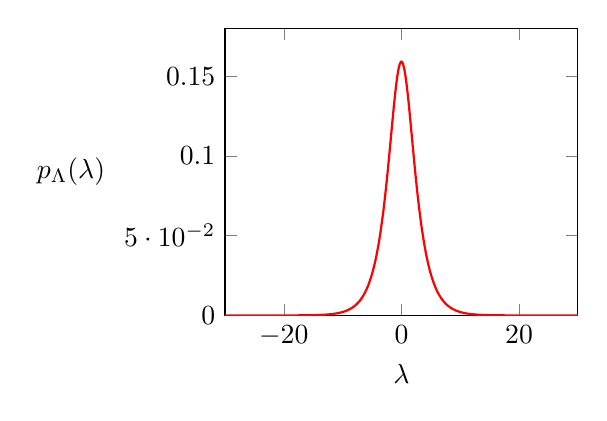
\begin{tikzpicture}
      \begin{axis}[
            xlabel=$\lambda$,
            ylabel=$p_\Lambda(\lambda)$,
            ylabel near ticks,
            xlabel near ticks,
            ylabel style={rotate=-90},
            xmin=-30,
            xmax=30,
            ymin=0,
            ymax=0.18,
            width=.5\linewidth]
      \addplot[color=red,thick,domain=-30:30,samples=300]{ (1 / cosh(x/2)) / (2 * pi * (2 / pi * rad(atan(exp(-0.5 * -30)))) - (2 / pi * rad(atan(exp(-0.5 * 30)))))};
      \end{axis}
      \end{tikzpicture}
      \caption{Probability density function $p_\Lambda(\lambda)$ for the same truncated continuous-time $\alpha$-cosine schedule as that in Figure \ref{fig:cosine_lambda_t}. The horizontal axis is the log signal-to-noise ratio $\lambda\in[\lambda_{\min}, \lambda_{\max}]$; the vertical axis is the corresponding probability density $p_\Lambda$.}
      \label{fig:p_lambda}
\end{figure}

The $\mathbf{v}$-prediction parameterisation loss given in Equation \ref{eq:v_parameterisation_loss} equates to the weighted loss $\mathcal{L}_w$ with:
\begin{align}
      w(\lambda)=\frac{1}{2\pi(t_1-t_0)}\exp\left(-\frac{\lambda}{2}\right)
\end{align}


\subsection{Reconstruction-Guided Sampling}
\label{sec:background_diffusion_reconstruction_guided_sampling}

\section{Climate Simulations}
\label{sec:background_climate}

% -----------------------------------------------------------------------------

\chapter{Results}
\label{chap:results}

% -----------------------------------------------------------------------------

\chapter{Conclusion}
\label{chap:conclusion}

% =============================================================================

% Finally, after the main matter, the back matter is specified.  This is
% typically populated with just the bibliography.  LaTeX deals with these
% in one of two ways, namely
%
% - inline, which roughly means the author specifies entries using the 
%   \bibitem macro and typesets them manually, or
% - using BiBTeX, which means entries are contained in a separate file
%   (which is essentially a databased) then inported; this is the 
%   approach used below, with the databased being dissertation.bib.
%
% Either way, the each entry has a key (or identifier) which can be used
% in the main matter to cite it, e.g., \cite{X}, \cite[Chapter 2}{Y}.
%
% We would recommend using BiBTeX, since it guarantees a consistent referencing style 
% and since many sites (such as dblp) provide references in BiBTeX format. 
% However, note that by default, BiBTeX will ixwgnore capital letters in article titles 
% to ensure consistency of style. This can lead to e.g. "NP-completeness" becoming
% "np-completeness". To avoid this, make sure any capital letters you want to preserve
% are enclosed in braces in the .bib, e.g. "{NP}-completeness".

\backmatter

\bibliography{dissertation}

% -----------------------------------------------------------------------------

% The dissertation concludes with a set of (optional) appendicies; these are 
% the same as chapters in a sense, but once signaled as being appendicies via
% the associated macro, LaTeX manages them appropriatly.

\appendix

\chapter{Diffusion Models}
\label{appx:diffusion}

\section{Derivation of $q(\mathbf{z}_t|\mathbf{z}_s)$}
\label{appx:diffusion_q_z_t_given_z_s}

From Equation \ref{eq:q_z_t_given_x}, we know $q(\mathbf{z}_t|\mathbf{x})$ is an isotropic Gaussian probability density function. As such, we can sample $\mathbf{z}_t\sim q(\mathbf{z}_t|\mathbf{x})$ by sampling $\boldsymbol\epsilon_t\sim\mathcal{N}(\mathbf{0}, \mathbf{I})$ from the multivariate standard Gaussian distribution and computing:
\begin{align}
      \mathbf{z}_t&=\alpha_t\mathbf{x}+\sigma_t\boldsymbol\epsilon_t\label{eq:z_t}
\end{align}
With some algebraic manipulation, we can show that:
\begin{align}
      \mathbf{z}_t&=\alpha_t\mathbf{x}+\sqrt{\sigma_t^2}\boldsymbol\epsilon_t\\
      &=\alpha_t\mathbf{x}+\sqrt{\sigma_t^2-\frac{\alpha_t^2}{\alpha_s^2}\sigma_s^2+\frac{\alpha_t^2}{\alpha_s^2}\sigma_s^2}\boldsymbol\epsilon_t\\
      &=\alpha_t\mathbf{x}+\sqrt{\sigma_t^2-\frac{\alpha_t^2}{\alpha_s^2}\sigma_s^2+\left(\frac{\alpha_t}{\alpha_s}\sigma_s\right)^2}\boldsymbol\epsilon_t
\end{align}
The sum of two independent Gaussian random variables with mean $\mu_1$ and $\mu_2$ and variance $\sigma_1^2$ and $\sigma_2^2$ is a Gaussian random variable with mean $\mu_1+\mu_2$ and variance $\sigma_1^2+\sigma_2^2$. As such, we can manipulate the above equation further to show that:
\begin{align}
      \mathbf{z}_t&=\alpha_t\mathbf{x}+\sqrt{\sigma_t^2-\frac{\alpha_t^2}{\alpha_s^2}\sigma_s^2}\boldsymbol\epsilon_t^*+\frac{\alpha_t}{\alpha_s}\sigma_s\boldsymbol\epsilon_s\\
      &=\alpha_t\mathbf{x}+\frac{\alpha_t}{\alpha_s}\sigma_s\boldsymbol\epsilon_s+\sqrt{\sigma_t^2-\frac{\alpha_t^2}{\alpha_s^2}\sigma_s^2}\boldsymbol\epsilon_t^*\\
      &=\frac{\alpha_s}{\alpha_s}\alpha_t\mathbf{x}+\frac{\alpha_t}{\alpha_s}\sigma_s\boldsymbol\epsilon_s+\sqrt{\sigma_t^2-\frac{\alpha_t^2}{\alpha_s^2}\sigma_s^2}\boldsymbol\epsilon_t^*\\
      &=\frac{\alpha_t}{\alpha_s}(\alpha_s\mathbf{x}+\sigma_s\boldsymbol\epsilon_s)+\sqrt{\sigma_t^2-\frac{\alpha_t^2}{\alpha_s^2}\sigma_s^2}\boldsymbol\epsilon_t^*\\
\end{align}
where $\boldsymbol\epsilon_t^*, \boldsymbol\epsilon_s\sim\mathcal{N}(\mathbf{0}, \mathbf{I})$ are similarly both sampled from the multivariate standard Gaussian distribution. We can substitute $\mathbf{z}_s=\alpha_s\mathbf{x}+\sigma_s\boldsymbol\epsilon_s$ into the above equation to show that:
\begin{align}
      \mathbf{z}_t&=\frac{\alpha_t}{\alpha_s}\mathbf{z}_s+\sqrt{\sigma_t^2-\frac{\alpha_t^2}{\alpha_s^2}\sigma_s^2}\boldsymbol\epsilon_t^*\\
      &=\alpha_{t|s}\mathbf{z}_s+\sigma_{t|s}\boldsymbol\epsilon_t^*\\
      &\sim\mathcal{N}\left(\mathbf{z}_t;\alpha_{t|s}\mathbf{z}_s,\sigma_{t|s}^2\mathbf{I}\right)
\end{align}
The subscript $t|s$ relates to the fact that $\alpha_{t|s}$ and $\sigma_{t|s}$ define the parameters of the Gaussian probability density function $q(\mathbf{z}_t|\mathbf{z}_s)$.

\section{$\alpha$-Cosine Noise Schedule}
\label{appx:diffusion_cosine_noise_schedule}

Before truncation, the continuous-time version of the $\alpha$-cosine schedule \cite{IDDPM_Nichol} as described in \cite{Simple_Diffusion_Hoogeboom} defines $\alpha_t^2$ at a given timestep $t\in[0,1]$ as:
\begin{align}
      \alpha_t^2=\cos^2\left(\frac{\pi}{2}t\right)
\end{align}
Since our model is a variance-preserving diffusion model, we can show that:
\begin{align}
      \sigma_t^2&=1-\alpha_t^2\\
      &=1-\cos^2\left(\frac{\pi}{2}t\right)\\
      &=\sin^2\left(\frac{\pi}{2}t\right)
\end{align}
As such, we define our noise schedule before truncation $\tilde{f}_\lambda$ for all $t\in[0,1]$ as:
\begin{align}
      \tilde{f}_\lambda(t)&=\log\left(\frac{\alpha_t^2}{\sigma_t^2}\right)\\
      &=\log\left(\frac{\cos^2\left(\frac{\pi}{2}t\right)}{\sin^2\left(\frac{\pi}{2}t\right)}\right)\\
      &=-2\log\left(\tan\left(\frac{\pi}{2}t\right)\right)
\end{align}
However, the above noise schedule means that $\tilde{f}_\lambda:[0,1]\to[-\infty, \infty]$; in simpler terms, $\lambda_t$ is unbounded. We follow prior work (e.g. \cite{Simple_Diffusion_Hoogeboom,VDM_Ho}) by truncating $\lambda_t$ to the desired range $[\lambda_{\min}, \lambda_{\max}]$. To do so, we first need to define the inverse of the unbounded noise schedule:
\begin{align}
      \tilde{f}_\lambda^{-1}(\lambda)=\frac{2}{\pi}\arctan\left(\exp\left(-\frac{1}{2}\lambda\right)\right)
\end{align}
From this, we define $t_0$ and $t_1$ as:
\begin{align}
      t_0&=\tilde{f}_\lambda^{-1}(0)=\frac{2}{\pi}\arctan\left(\exp\left(-\frac{1}{2}\lambda_{\max}\right)\right)\\
      t_1&=\tilde{f}_\lambda^{-1}(1)=\frac{2}{\pi}\arctan\left(\exp\left(-\frac{1}{2}\lambda_{\min}\right)\right)
\end{align}
The truncated noise schedule used in this work is then defined as:
\begin{align}
      f_\lambda(t)&=\tilde{f}_\lambda(t_0+t(t_1-t_0))\\
      &=-2\log\left(\tan\left(\frac{\pi}{2}(t_0+t(t_1-t_0))\right)\right)
\end{align}

\section{$\mathbf{v}$-Prediction Parameterisation}
\label{appx:diffusion_v_prediction_parameterisation}

From Equation \ref{eq:z_t}, for a given datapoint $\mathbf{x}\sim q(\mathbf{x})$, we can sample latent variable $\mathbf{z}_t\sim q(\mathbf{z}_t|\mathbf{x})$ via:
\begin{align}
      \mathbf{z}_t=\alpha_t\mathbf{x}+\sigma_t\boldsymbol\epsilon
\end{align}
where $\boldsymbol\epsilon\sim\mathcal{N}(\mathbf{0},\mathbf{I})$ is multivariate standard Gaussian noise. We define the velocity of $\mathbf{z}_t$ as
\begin{align}
      \mathbf{v}_t=\frac{d\mathbf{z}_t}{d \psi}
\end{align}
i.e. the derivative of $\mathbf{z}_t$ with respect to $\psi$, which itself is:
\begin{align}
      \psi_t&=\arctan\left(\frac{\sigma_t}{\alpha_t}\right)\\
      &=\arctan\left(\frac{\sin\left(\frac{\pi}{2}(t_0+t(t_1-t_0))\right)}{\cos\left(\frac{\pi}{2}(t_0+t(t_1-t_0))\right)}
      \right)\\
      &=\arctan\left(\tan\left(\frac{\pi}{2}(t_0+t(t_1-t_0))\right)\right)\\
      &=\frac{\pi}{2}(t_0+t(t_1-t_0))
\end{align}
when using the truncated continuous-time $\alpha$-cosine noise schedule as per Section \ref{sec:background_diffusion_noise_schedule}. As such, we can formulate the velocity as:
\begin{align}
      \mathbf{v}_t=\frac{\mathbf{z}_t}{d\psi}&=\frac{d\cos(\psi)}{d\psi}\mathbf{x}+\frac{d\sin(\psi)}{d\psi}\boldsymbol\epsilon\\
      &=-\sin(\psi)\mathbf{x}+\cos(\psi)\boldsymbol\epsilon\\
      &=\alpha_t\boldsymbol\epsilon-\sigma_t\mathbf{x}\label{eq:v_t_equals_alpha_t_epsilon_minus_sigma_t_x}
\end{align}
We can rearrange the above to derive a form for $\mathbf{x}$ in terms of $\mathbf{z}_t$ and $\mathbf{v}_t$ as follows:
\begin{align}
      \mathbf{v}_t&=-\sin(\psi)\mathbf{x}+\cos(\psi)\boldsymbol\epsilon\\
      \sin(\psi)\mathbf{x}&=\cos(\psi)\boldsymbol\epsilon-\mathbf{v}_t\\
      &=\cos(\psi)\left(\frac{\mathbf{z}_t-\cos(\psi)\mathbf{x}}{\sin(\psi)}\right)-\mathbf{v}_t\\
      \sin^2(\psi)\mathbf{x}&=\cos(\psi)\mathbf{z}_t-\cos^2(\psi)\mathbf{x}-\sin(\psi)\mathbf{v}_t\\
      \sin^2(\psi)\mathbf{x}+\cos^2(\psi)\mathbf{x}&=\cos(\psi)\mathbf{z}_t-\sin(\psi)\mathbf{v}_t\\
      (\sin^2(\psi)+\cos^2(\psi))\mathbf{x}&=\cos(\psi)\mathbf{z}_t-\sin(\psi)\mathbf{v}_t\\
      \mathbf{x}&=\cos(\psi)\mathbf{z}_t-\sin(\psi)\mathbf{v}_t\\
      &=\alpha_t\mathbf{z}_t-\sigma_t\mathbf{v}_t
\end{align}
As per Equation \ref{eq:v_t_equals_alpha_t_epsilon_minus_sigma_t_x}, during training we can 



We define the velocity of $\mathbf{z}_t$ as 

We rearrange to get:

As such:
\begin{align}
      \mathbf{x}=\alpha_t\mathbf{z}_t-\sigma_t\mathbf{v}_t
\end{align}

During training, we train the model to minimise:
\begin{align}
      \mathbb{E}_{\mathbf{x},\boldsymbol\epsilon, t}\left[\Vert\mathbf{v}_t-\hat{\mathbf{v}}_\theta(\mathbf{z}_t, \lambda_t)\Vert_2^2\right]
\end{align}

\section{Relationship Between the ELBO and Weighted Loss}
\label{appx:diffusion_elbo_weighted_loss}

\begin{align}
      \log p_\theta(\mathbf{x})&=\mathbb{E}_{\mathbf{z}\sim q(\mathbf{z}|\mathbf{x})}\left[\log p_\theta(\mathbf{x})\right]\\
      &=\mathbb{E}_{\mathbf{z}\sim q(\mathbf{z}|\mathbf{x})}\left[\log\left(\frac{p_\theta(\mathbf{x},\mathbf{z})}{p_\theta(\mathbf{z}|\mathbf{x})}\right)\right]\\
      &=\mathbb{E}_{\mathbf{z}\sim q(\mathbf{z}|\mathbf{x})}\left[\log\left(\frac{p_\theta(\mathbf{x},\mathbf{z})q(\mathbf{z}|\mathbf{x})}{p_\theta(\mathbf{z}|\mathbf{x})q(\mathbf{z}|\mathbf{x})}\right)\right]\\
      &=\mathbb{E}_{\mathbf{z}\sim q(\mathbf{z}|\mathbf{x})}\left[\log\left(\frac{p_\theta(\mathbf{x},\mathbf{z})}{q(\mathbf{z}|\mathbf{x})}\right)\right]+\mathbb{E}_{\mathbf{z}\sim q(\mathbf{z}|\mathbf{x})}\left[\log\left(\frac{q(\mathbf{z}|\mathbf{x})}{p_\theta(\mathbf{z}|\mathbf{x})}\right)\right]\\
      &=\mathbb{E}_{\mathbf{z}\sim q(\mathbf{z}|\mathbf{x})}\left[\log\left(\frac{p_\theta(\mathbf{x},\mathbf{z})}{q(\mathbf{z}|\mathbf{x})}\right)\right]+D_{KL}(q(\mathbf{z}|\mathbf{x})\Vert p_\theta(\mathbf{z}|\mathbf{x}))\\
      &\ge \mathbb{E}_{\mathbf{z}\sim q(\mathbf{z}|\mathbf{x})}\left[\log\left(\frac{p_\theta(\mathbf{x},\mathbf{z})}{q(\mathbf{z}|\mathbf{x})}\right)\right]\\
      &=\mathbb{E}_{\mathbf{z}\sim q(\mathbf{z}|\mathbf{x})}\left[\log\left(\frac{p_\theta(\mathbf{x}|\mathbf{z})p_\theta(\mathbf{z})}{q(\mathbf{z}|\mathbf{x})}\right)\right]\\
      &=\mathbb{E}_{\mathbf{z}\sim q(\mathbf{z}|\mathbf{x})}\left[\log p_\theta(\mathbf{x}|\mathbf{z})\right]+\mathbb{E}_{\mathbf{z}\sim q(\mathbf{z}|\mathbf{x})}\left[\log\left(\frac{p_\theta(\mathbf{z})}{q(\mathbf{z}|\mathbf{x})}\right)\right]\\
      &=\mathbb{E}_{\mathbf{z}\sim q(\mathbf{z}|\mathbf{x})}\left[\log p_\theta(\mathbf{x}|\mathbf{z})\right]-\mathbb{E}_{\mathbf{z}\sim q(\mathbf{z}|\mathbf{x})}\left[\log\left(\frac{q(\mathbf{z}|\mathbf{x})}{p_\theta(\mathbf{z})}\right)\right]\\
      &=\mathbb{E}_{\mathbf{z}\sim q(\mathbf{z}|\mathbf{x})}\left[\log p_\theta(\mathbf{x}|\mathbf{z})\right]-D_{KL}(q(\mathbf{z}|\mathbf{x})\Vert p_\theta(\mathbf{z}))\\
      &=\mathbb{E}_{\mathbf{z}\sim q(\mathbf{z}|\mathbf{x})}\left[\log p_\theta(\mathbf{x}|\mathbf{z})\right]-D_{KL}(q(\mathbf{z}|\mathbf{x})\Vert p_\theta(\mathbf{z}))\\
      &=\mathbb{E}_{\mathbf{z}\sim q(\mathbf{z}|\mathbf{x})}\left[\log p_\theta(\mathbf{x}|\mathbf{z})\right]-D_{KL}(q(\mathbf{z}_1|\mathbf{x})\Vert p_\theta(\mathbf{z_1}))-\int_{\lambda_{\min}}^{\lambda_{\max}}\frac{d}{d\lambda}
\end{align}

% =============================================================================

\end{document}
